\newpage
\section{Praktikum 2 - Teil I: Informationsextraktion und Textzerlegung}

\subsection{HANA VM}

{\color{MidnightBlue}
\begin{lstlisting}
connection = dbapi.connect('192.168.56.102', 39041, 'SYSTEM', 'Password1')
\end{lstlisting}}

\subsection{Tabellen}

{\color{MidnightBlue}
\begin{lstlisting}[language=SQL]
CREATE TABLE GRAPPLING_INSIDER_CONTENT(
    url VARCHAR(300) PRIMARY KEY,
    title VARCHAR(300),
    text NCLOB MEMORY THRESHOLD 1000
)
CREATE TABLE GRAPPLING_INSIDER_CATEGORIES(
    url VARCHAR(300),
    category VARCHAR(30)
)
CREATE TABLE GRAPPLING_INSIDER_EXTERNAL_LINKS(
    url VARCHAR(300),
    external_link_url NCLOB MEMORY THRESHOLD 1000,
    external_link_text VARCHAR(700)
)
\end{lstlisting}}

\subsection{Füllen der DB}

{\color{MidnightBlue}
\begin{lstlisting}[language=SQL]
INSERT INTO GRAPPLING_INSIDER_CONTENT (url, title, text) VALUES (?,?,?)
INSERT INTO GRAPPLING_INSIDER_CATEGORIES (url, category) VALUES (?,?)
INSERT INTO GRAPPLING_INSIDER_EXTERNAL_LINKS (url, link_url, link_text) VALUES (?,?,?)
\end{lstlisting}}

\subsection{Prüfen}

Alle Daten wie erwartet in der Datenbank.

\subsection{Text-Index}

{\color{MidnightBlue}
\begin{lstlisting}[language=SQL]
CREATE FULLTEXT INDEX "GRAPPLING_INSIDER_INDEX"
ON "SYSTEM"."GRAPPLING_INSIDER_CONTENT" ("TEXT")
CONFIGURATION 'LINGANALYSIS_FULL'
ASYNC LANGUAGE DETECTION ('en')
TEXT ANALYSIS ON
\end{lstlisting}}

\subsection{Text-Index prüfen}

Es standen drei Indexarten zur Auswahl:
\begin{itemize}
	\item LINGANALYSIS\_BASIC: Tokenisierung mit unter anderem Erkennung der Sprache, Normalisierung (bei uns nur forced lower-case), Paragraphen- und Satzindex, sowie Offset im Dokument.
	\item LINGANALYSIS\_STEMS: Hier werden noch die Lemmatisierungen der Tokens hinzugefügt, was bei uns nur mangelhaft funktionierte. Im Satz den wir uns angeschaut haben war nur das Entfernen von \texttt{s} am Wortende bei Mehrzahl (zB \texttt{friends} zu \texttt{friend}) aufzufinden, alles andere hat gefehlt (zB \texttt{confined} zu \texttt{confine}).
	\item LINGANALYSIS\_FULL: Zuvor wurde der Token Typ nur zwischen \texttt{punctuation} und allen anderen unterschieden. Bei dieser Einstellung kommt die restliche PoS Analyse dazu. Dies funktionierte grö\ss{}tenteils gut.
\end{itemize}

\noindent Die Lemmatisierung (TA\_STEM) war in unserem Fall nicht nutzbar und wir wissen nicht woran es lag, bzw. ob wir darauf hätten Einfluss nehmen können. Die PoS Analyse (TA\_TYPE) war zufriedenstellend und könnte nur noch einmal mit Kontext wichtigen Bedeutungen korrigiert werden, wie man bei späteren Analysen sieht. Bei unseren Daten wären das zum Beispiel Namen wie \texttt{Jiu Jitsu} (Sport) oder dem \texttt{Gi} (Kleidung) als \texttt{proper name} zu definieren, statt wie hier häufig als Adjektive.

\setcounter{section}{1}
\section{Praktikum 2 - Teil II: Reporting auf zerlegten Texten}

\subsection{Worthäufigkeiten (Nomen) pro Dokument}

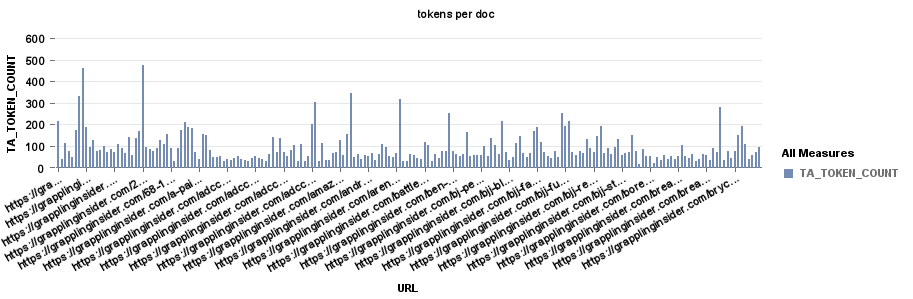
\includegraphics[width=\textwidth]{images/tokens_per_doc.png}

\subsection{Lexikon}

{\color{MidnightBlue}
\begin{lstlisting}
lexicon length: 26936 tokens
filtered lexicon length: 25525 tokens
average document length: 525 tokens
average sentence length: 23 tokens
\end{lstlisting}}

\subsection{Verteilung der Worthäufigkeiten}

\noindent Auf Nomen beschränkt: \\

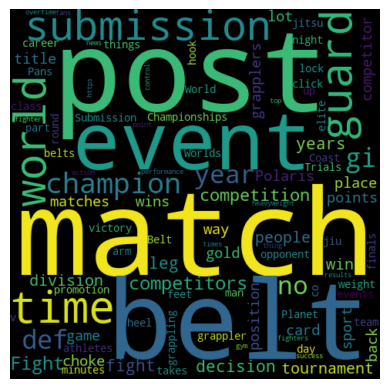
\includegraphics[width=0.5\textwidth]{images/top_100_wordcloud.png}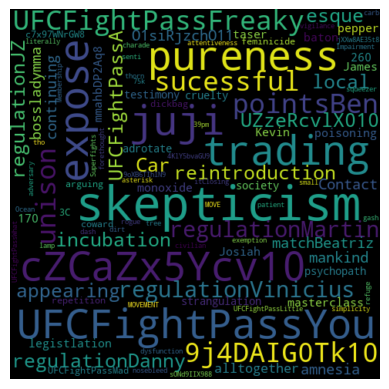
\includegraphics[width=0.5\textwidth]{images/bottom_100_wordcloud.png} \\

\noindent Die top 100 Tokens der WordCloud sehen sehr wie erwartet aus, ohne Überraschungen. Die bottom 100 Tokens sind gro{\ss}teils Unsinn und besteht aus Worten die nur ein mal vorkommen. Es gibt deutlich mehr als 100 Tokens die nur ein mal vorkommen, somit ist die Auswahl auch sehr willkürlich \\

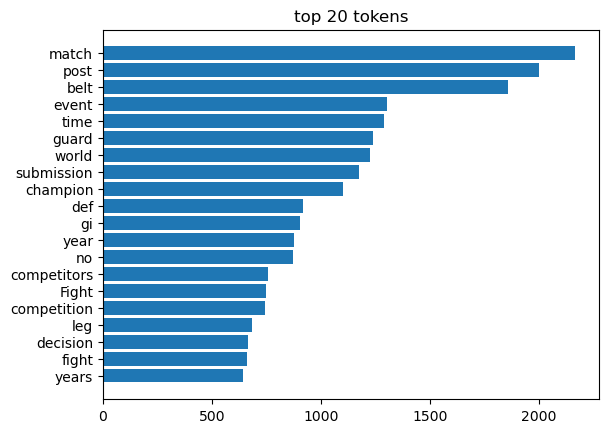
\includegraphics[width=0.5\textwidth]{images/top_20_tokens.png}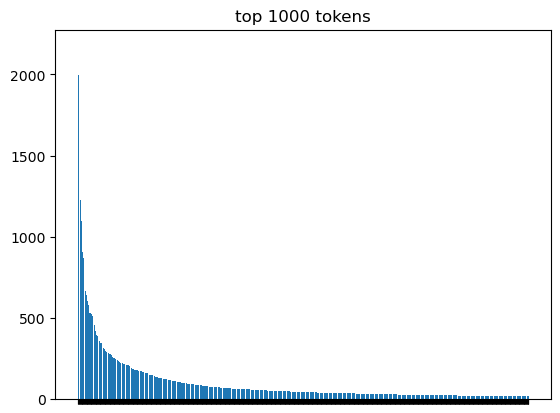
\includegraphics[width=0.5\textwidth]{images/top_1000_tokens.png} \\

\noindent Die top 20 tokens sind auch nicht überraschend. Bei einer Darstellung der top 1000 tokens erkennt man, dass das Zipfsche Gesetz grob gelten könnte.

\subsection{Mehrdeutigkeit}

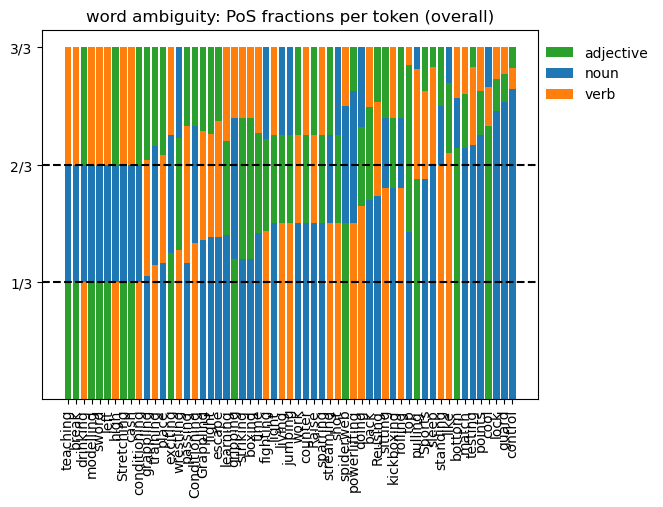
\includegraphics[width=\textwidth]{images/word_ambiguity.png} \\

\noindent In diesem Plot sind die mehrdeutigsten Worte dargestellt. \texttt{teaching} wird beispielsweise genau gleich oft als Verb, Adjektiv und Nomen gebraucht. \texttt{control} hingegen wird über $\frac{5}{6}$ mal als Nomen gebraucht und nur etwa jeweils $\frac{1}{12}$ mal als Adjektiv oder Verb.

\subsection{Weitere Statistiken und Visualisierungen}

{\color{MidnightBlue}
\begin{lstlisting}
url count: 1375
categories: ['ADCC News', 'Academies', 'BJJ Culture', 'BJJ History',
	'BJJ Injury', 'BJJ News', 'COVID', 'Celebrity', 'Conditioning',
	'Endurance', 'Featured', 'Fitness', 'Health', 'IBJJF News',
	'Interview', 'Judo News', 'MMA News', 'Media', 'Opinion',
	'Preview Events', 'Review Events', 'Reviews', 'Technique',
	'UK BJJ News', 'Uncategorized', 'Video', 'Wellbeing',
	'White belt', "Women's BJJ News", 'Wrestling News']
categories count: 30
\end{lstlisting}}

\noindent Als weitere Statistiken haben wir uns die Anzahl an Artikeln und die Kategorien samt Anzahl derer ausgeben lassen.

